\chapter{Diffraction}

\chapter{Fraunhofer and Fresnel Diffraction}

\section{Fraunhofer Diffraction}

\begin{figure}[H]
  \centering
  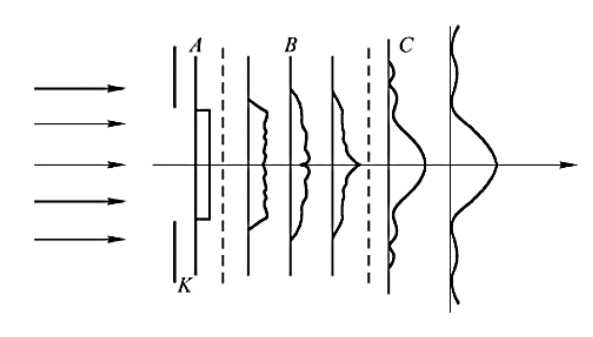
\includegraphics[width=0.6\linewidth]{figures/Fraunhofer-Fresnel-Diffraction}
\end{figure}

\begin{figure}[H]
  \centering
  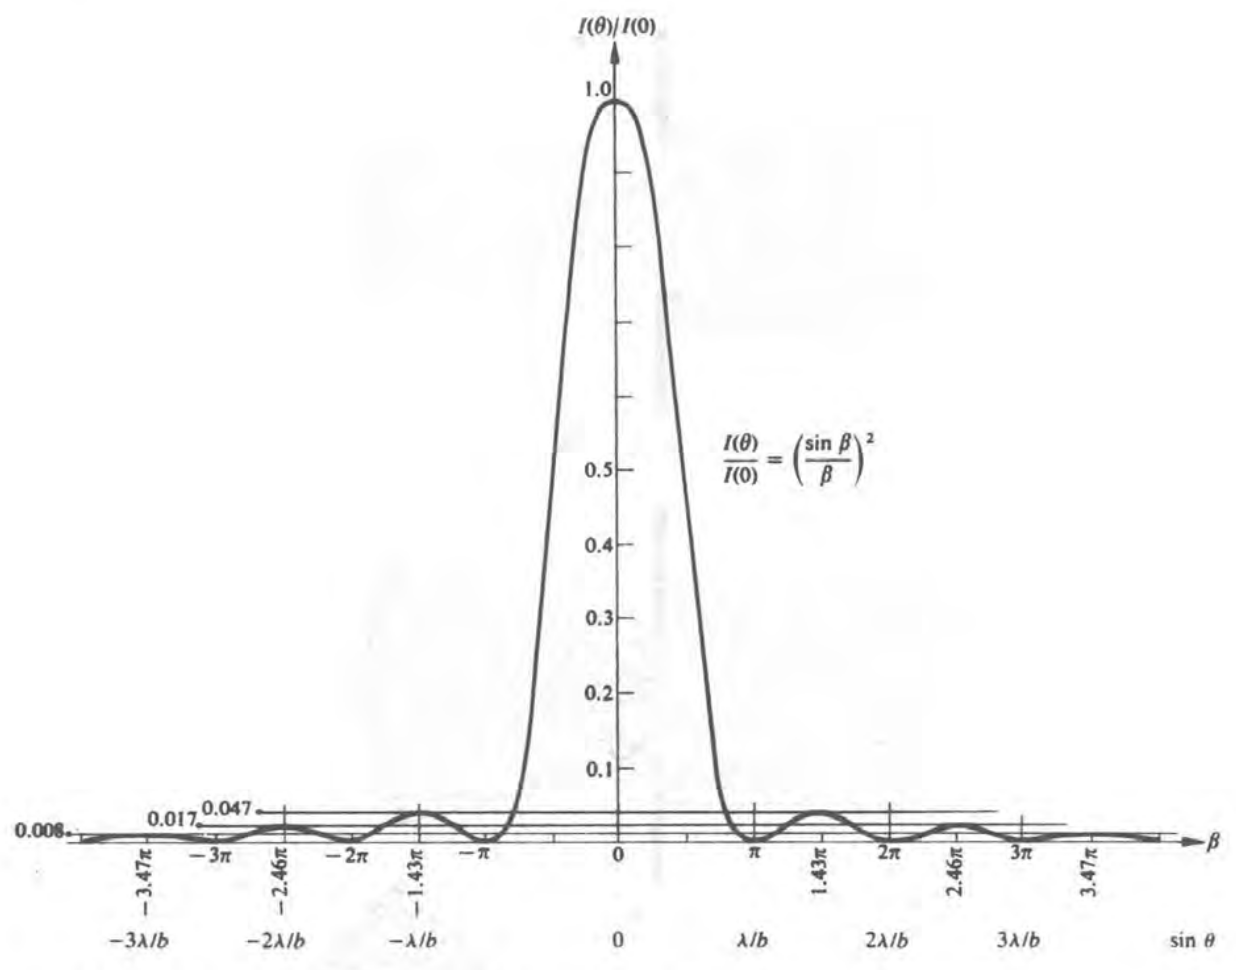
\includegraphics[width=0.7\linewidth]{figures/Fraunhofer-Diffraction-Irradance}
\end{figure}

White fringes:

\begin{equation*}
  \left\{
    \begin{aligned}
      b \sin \theta &= 0 && \quad\quad \text{Central Fringe} \\
      \sin \theta &= \pm \left( 2 m + 1 \right) \cdot \dfrac{\lambda}{2b} && \quad\quad m = 1,2,3,\dots
    \end{aligned}
  \right.
  \quad\quad 
  \left\{
    \begin{aligned}
      \Delta \theta_0 &= 2 \cdot \dfrac{\lambda}{b} \\
      \Delta \theta &= \dfrac{\lambda}{b} 
    \end{aligned}
  \right.
\end{equation*}

Dark fringes:

\begin{equation*}
  \begin{aligned}
    \sin \theta = \pm m \cdot \dfrac{\lambda}{b} \quad\quad m = 1,2,3,\dots
  \end{aligned}
\end{equation*}



%%% Local Variables:
%%% mode: latex
%%% TeX-master: "Optics"
%%% End:
